%!TEX root = report.tex

The program was started by following the instructions on the borg wiki, after which we ran \t{roslaunch navigation exercise7.launch}. This started the correct map in RViz, which can be seen in \ref{fig:1:map}, as well as started the other requirements. The robot was then given goals by setting a \t{2D nav goal} in RViz.

\begin{figure}[h!]
	\centering
	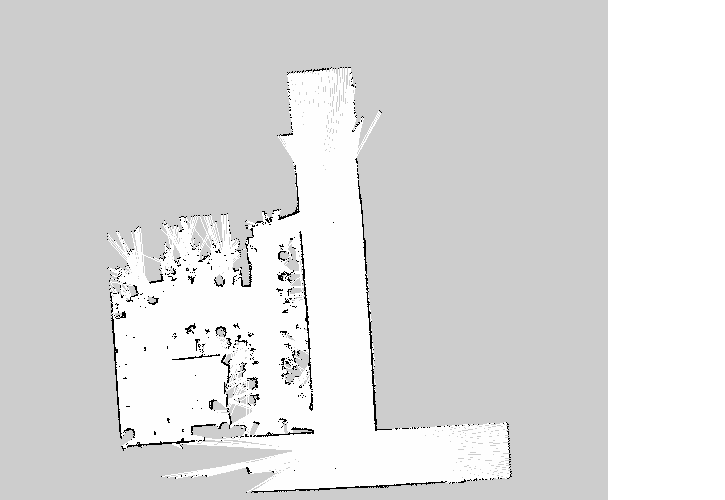
\includegraphics[width=\textwidth]{./img/real_lab.png}
	\caption{The map that was made of the lab through mapping with Alice using the teleop keyboard package.}
	\label{fig:1:map}
\end{figure}

We had several interesting findings. First of all, real life is a lot different than a simulation.

An incremental approach was decided upon in order to try and reach the final goal, which was to drive the robot from the entrance of the lab back to its normal standing position. First the robot was driven from 1 end of the hall to the other, to try and understand what the robot saw and most of all, if the navigation worked and if adjustments had to be made. 

Afterwards we attempted to drive Alice to the middle of the lab, at the T-split of the paths. We found a few issues. The main one was that Alice thought the door wasn't big enough to her to fit through, meaning that it couldn't even get into the class. 

Another very annoying problem was random students walking through the hall. The robot would see them approaching as obstacles, and save them as an obstacle in its global as well as local cost map. The local cost map would get updated or regenerated, meaning the students would dissapear from nearby, but the reading further away would remain. The reason this was negative for Alice was due to its planning algorithm. Alice plans a route based on its findings and memory, so if it has seen obstacles further away, then it would take those into account for its planning, even though the students had long since dissapeared. This caused it to not be able to find a route quite a few times.

In the end we went for the solution of placing Alice in front of the lab door, so that it could already see a bit into the lab. This caused it to have less trouble from student, as well as make it see that driving through an open door was, in fact, possible. This worked and then Alice got to the T-split on its own, where it spinned in order to get the correct angle that we had set. Unfortunately the chairs in the lab messed up the local costmap quite a bit, causing it to have issues with the mapping. 

There we restarted \t{exercise7.launch} and gave it its final goal, which was the original position in the pit. Alice drove straight forward towards the white board, but tried to cut the corner a bit too steep which caused it to get stuck near Maikel and Sybren's PC. We didn't have any time left on Alice, unfortunately, otherwise we would've attempted to change its path finding a tad in order to take more room when clearing corners.